\documentclass{spaexp}
\major{物理学}
\name{}
\grade{2017级}
\stuid{17353038}
\exptitle{E1\quad 高温超导实验}

\graphicspath{{img/}}

\begin{document}
    \maketitle
    
    \section{背景介绍}
    \section{实验原理}
        \subsection{实验目的}
        \subsection{超导(左广信)}
            \subsubsection{超导}
                当温度降低到超导相变温度时,超导材料将会相变为超导态,具有两个特征:一是零电阻,二是完全抗磁性(迈斯纳效应)。
                超导体的超导态相变及维持需要三个临界条件,一是温度降低到临界温度$T_c$,二是外部磁场强度低于临界磁场强度$H_c$,三是超导体传导的电流密度低于临界电流密度$J_c$。
                超导体又包括I类超导体与II类超导体。I类超导体在外界磁场强度超过$H_c$后内部磁场发生突变退出超导态,
                而II类超导体在外部磁场强度超过下临界磁场强度$H_{c1}$后内部磁场强度不为零,部分磁感线穿透材料,处于混合态;
                随着外加磁场强度升高穿透材料的磁感线亦增多,当外部磁场强度超过上临界磁场强度$H_{c2}$后磁感线完全穿透,超导态过渡到一般态。
                超导体与理想导体都可具有零电阻特性,但是超导体与理想导体的区别在于超导体还具有完全抗磁性。
                超导体的完全抗磁性是指当超导材料相变为超导态后,在超导体内部完全没有磁感线穿过,超导体内部磁场为零。
                且这种完全抗磁性只依赖于是否处于超导态这一热力学状态,换言之,不论超导体内部事先有没有磁场,一旦进入超导态,其内部再无磁感线穿过。
                故而可以在实验中通过检测超导体外部磁场变化来判断材料是否进入超导,从而测得相变温度。
            \subsubsection{超导零电阻的BCS解释}
                电子只有两种自旋,即$S= \pm 1/$,在超导材料中,自旋与动量相反的两个电子可以形成库珀对,而库珀对在晶格中可以无损耗地运动,
                唯象地解释这是因为当电子临近原子核时,将凭借自身的负电荷吸引附近的核正电荷,而受吸引后向电子位移了一部分的核正电荷们将形成一个高电势区,
                继而吸引另一个自旋与先前电子相反的电子与之形成一个配对,凝结为库珀对。与当温度足够低时,晶格原子的振动(声子)能量会低于库珀对的结合能,
                从而库珀对与晶格无法交换能量,电子对们凝聚为一个集体,在超导体中集体运动,此时没有电阻,即为零电阻超导态.但是这种解释局限于I类超导体,
                并不能很好地解释II类超导体的成因。

            \subsubsection{迈斯纳效应的物理解释}
                严格来说,处于超导态的超导体内部,磁感线不能大范围的存在。
                产生完全抗磁性的原因是:当材料处于超导态时,在磁场的作用下材料表面将会产生一个无损感应电流,且这个电流的磁效应刚好抵消了外界磁场,导致超导体内部无磁感线穿过。
                迈斯纳效应是超导体不同于理想导体的特性。我们可以根据麦克斯韦方程组推导理想导体内部磁感应强度B随外界磁场变化的关系:
                根据$\nabla \times E = -\partial B / \partial t$, 且$E=\rho J$, 其中$\rho$为电阻率,对于理想导体$\rho=0$,从而$E=0$,因而磁感应强度B的随时变化率为0,
                从而我们得知,对于理想导体,加磁场前后导体内部的磁感应强度不变.这一点是与超导体的迈斯纳效应不同的.

        \subsection{降温与保温(张旭盈)}
            \subsubsection{低温的获得}
                取决于制冷和隔热两个因素。
                \begin{description}
                    \item[制冷:]从物体中抽走热量使其冷却。
                    \item[隔热:]阻碍物体和外界产生热量交换。
                \end{description}
                当外界给予物体的热量等于制冷抽走的热量时,物体达到热平衡即温度不再发生变化。
                
            \subsubsection{常用隔热方式:真空}
                \begin{description}
                    \item[热传导的三种方式:]传导、对流、辐射
                    在真空中热传导和对流可以忽略不计,只有热辐射传热。
                    \item[减少热辐射的方法:]采用低温防辐射屏或多层绝热材料。
                \end{description}
            \subsubsection{防辐射屏的效果计算}
                设物体温度为$T_L$,环境温度为$T_E$,防辐射屏温度为$T_M$。$\Delta Q$为单位时间单位面积的净传热。
                无防辐射屏时,物体与环境之间的净传热:$\Delta Q = \sigma(T_E^4 - T_L^4)$
                有防辐射屏时,物体与屏、屏与环境的净传热:
                $$\Delta Q_1 = \sigma(T_E^4 - T_M^4)$$
                $$\Delta Q_2 = \sigma(T_M^4 - T_L^4)$$
                防辐射屏达到热平衡:
                $$\Delta Q_1 = \sigma(T_E^4 - T_M^4) = \Delta Q_2 = \sigma(T_M^4 - T_L^4) = \frac12 \Delta Q$$
                所以从环境到物体的净传热减半。
            \subsubsection{低温恒温器}
                \begin{description}
                    \item[本实验采用:]漏热式低温恒温器
                    \item[恒温器实现温度控制的方法:]冷源和热源漏热在某一温度下达到平衡。
                    \item[冷源漏热:]冷源与冷端热接触(隔热采用真空技术并设置防辐射屏保证效果。)
                    \item[热源漏热:]在冷源热通道(冷颈)进行加热补偿。
                \end{description}
                
            \subsubsection{制冷及装置}
                本实验中的两种制冷方式:制冷剂(液氮)、循环制冷机
                \begin{itemize}
                    \item 液氮+恒温器:液氮恒温器
                    液氮可以在低温下汽化吸热,达到制冷的目的。
                    通过加注液氮冷却样品,期间中心杆可以帮助控制液氮流速;控温仪会通过加热器控制温度到稳定值实现控温。
                    \item 循环制冷机+恒温器:制冷恒温器
                    压缩机提供常温高压氦气,在冷头经过降温后膨胀吸热冷却样品,再度回到压缩机,实现循环制冷。
                    控温仪通过加热器实现控温。
                    \item 两者制冷的前提:真空环境
                \end{itemize}
        \subsection{数据采集与分析}
            \subsubsection{电阻测量(梁伟德)}
            实验中需要测量材料的电阻作为进入超导态的判断条件。测量接近0的小电阻需要四引线法\autoref{img:四引线测电阻电路原理图}。同时,还需考虑电阻由于不对称而引起的电势差:
            温差电势$V_T$,接触电势$V_C$。若使用直流电流进行测量,则有测量结果:$V_+ = IR + V_C + V_T$,为消除温差电势与接触电势,
            需要再进行一次反向电流的测量:$V_- = -IR + V_C + V_T$,可以得到:
            \begin{equation}
                R = \frac{V_+ - V_-}{2I}
            \end{equation}

            \begin{figure}
                \ct
                \caption{四引线测电阻电路原理图}
                \label{img:四引线测电阻电路原理图}
                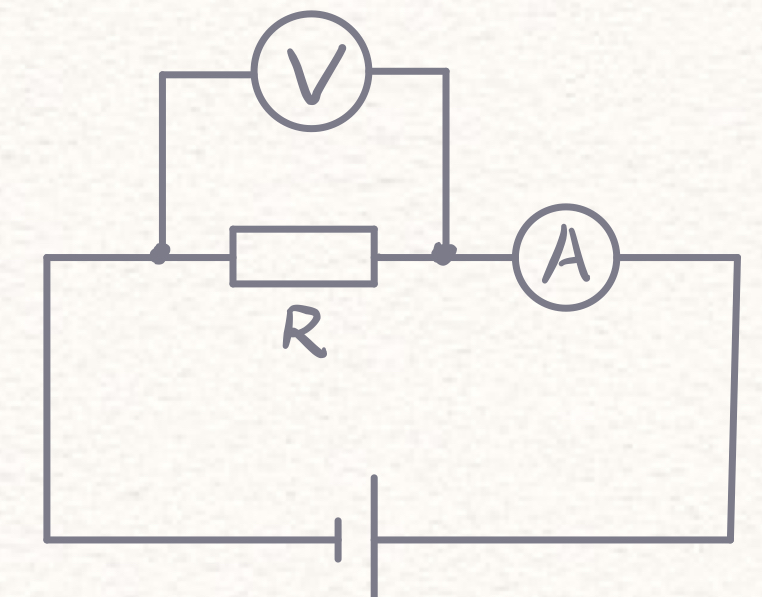
\includegraphics[width = 0.4\textwidth]{fourfoot.jpeg}
            \end{figure}

            实际测量时,变换两次电流方向分别测量,得到一个测量电阻值。在实验配备 IT6411S 可编程直流恒流源,可以通过计算机控制实现。\par

            为消除温差电势与接触电势,还可以使用{\bf{交流四引线测量法}},由交流电的特性可以直接排除直流电势的影响。使用锁相放大器测量弱小电阻是一个较好的选择。\autoref{img:锁相放大器实现交流四引线电阻测量}
            利用锁相功能不仅能排除直流噪声,还能排除其他高频噪声。\par

            使用交流电源对超导系统进行供电,讲电阻两侧用四引线接入锁相放大器的SIGNAL IN中则可以得到电阻两侧电势差,最终计算出超导材料的电阻。
            \begin{figure}
                \ct
                \caption{锁相放大器实现交流四引线电阻测量}
                \label{img:锁相放大器实现交流四引线电阻测量}
                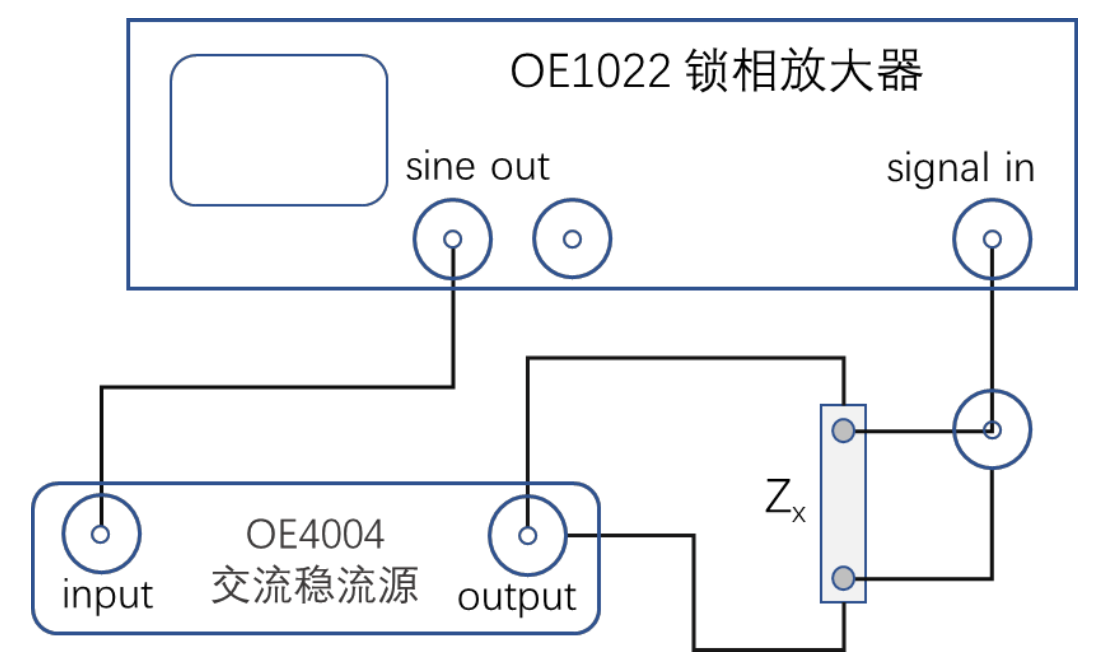
\includegraphics[width = 0.7\textwidth]{dcfourfoot.png}
            \end{figure}


            \subsubsection{测量交流磁化率(梁伟棠)}
                根据电磁理论,在恒定外磁场下,介质对磁场对响应定义了磁化率$\chi$,如式\eqref{MXH}。
                \begin{equation}
                    M = \chi H
                    \label{MXH}
                \end{equation}
                假设外磁场以准静止态发生变化,即任一时刻式\eqref{MXH}仍成立,则任意两时刻的差值有式\eqref{acMXH}。
                \begin{equation}
                    M'-M=\chi(H'-H)\leftrightarrow \Delta M = \chi \Delta H
                    \label{acMXH}
                \end{equation}
                因此小范围内交变磁场的准静止态变化,交流磁化率$\tilde{\chi}$可参照\eqref{acMXH}定义为
                \begin{equation}
                    \tilde{\chi} = \dfrac{\partial M}{\partial H}
                    \label{acchi}
                \end{equation}
                交流磁化率通过一对互感线圈,产生磁场的线圈叫初级线圈,测量感应电动势的线圈叫次级线圈。次级线圈的感应电动势与线圈内部磁感应强度$\tilde{B}$的变化率成正比
                \begin{equation}
                    \tilde{\varepsilon} = k_1\dfrac{\partial \tilde{B}}{\partial t}
                \end{equation}
                由电磁理论$\tilde{B}=\mu_0 (\tilde{H}+\tilde{M})$,感应电动势可以改写成
                \begin{equation}
                    \tilde{\varepsilon} = k_1 \mu_0(1+\tilde{\chi})\dfrac{\partial \tilde{H}}{\partial t}
                \end{equation}
                而磁场强度$H$与通过其线圈的电流$\tilde{I}$成正比。
                \begin{equation}
                    \tilde{\varepsilon} = k_1 k_2 \mu_0(1+\tilde{\chi})\dfrac{\partial \tilde{I}}{\partial t}
                \end{equation}
                由此交流磁化率由
                \begin{equation}
                    \tilde{\chi} = \dfrac{\tilde{\varepsilon}}{k_1 k_2\mu_0 \dfrac{\partial \tilde{I}}{\partial t}} - 1
                    \label{meachi}
                \end{equation}
                由式\eqref{meachi},因为感应电动势$\tilde{\varepsilon}$和电流$\tilde{I}$是复数,所以交流磁化率$\tilde{\chi}$也是复数。
                \begin{equation}
                    \tilde{\chi} = \chi ' +\chi ''
                    \label{complexchi}
                \end{equation}
                同时,只要知道了感应电动势$\tilde{\varepsilon}$和电流$\tilde{I}$也就知道了交流磁化率$\tilde{\chi}$,这就是测量交流磁化率的方法。
                \begin{figure}[h]      
                    \centering 
                    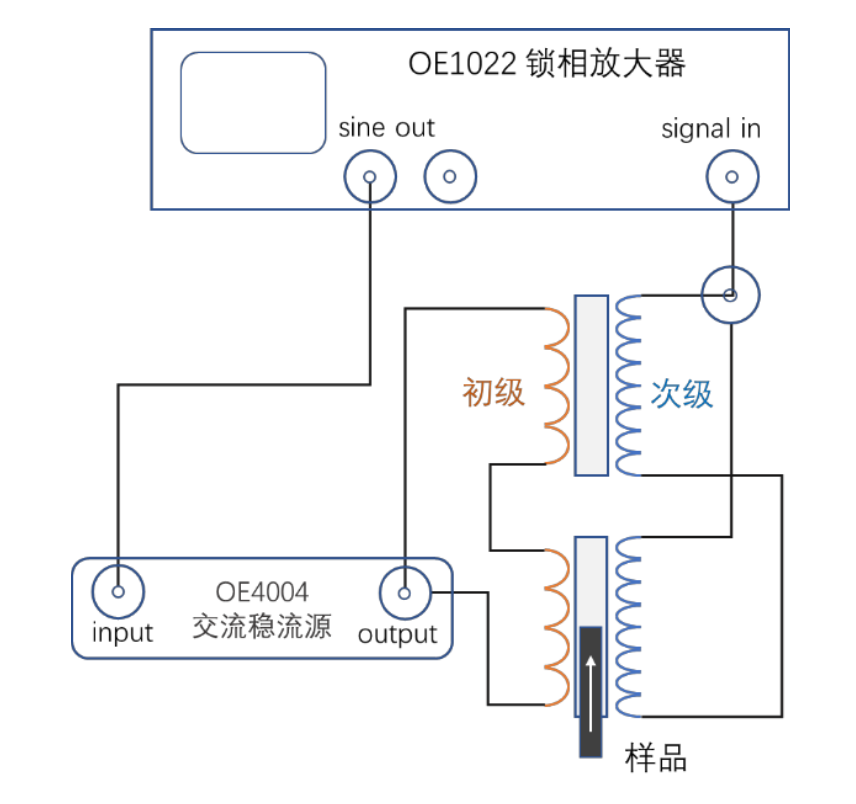
\includegraphics[width=0.5\textwidth]{meachi.png}
                    \caption{差分法测量交流磁化率}\label{chafen}
                    
                \end{figure}
                
                图\autoref{chafen} 提供了测量交流磁化率的电路图,这里还做了改进,通过并联一组线圈,然后将放入被测样品的线圈的信号减去不放入样品的线圈的信号,来抵消线圈产生的信号$k_1k_2\mu_0\dfrac{\partial \tilde{I}}{\partial t}$。因为线圈的信号$k_1k_2\mu_0\dfrac{\partial \tilde{I}}{\partial t}$远强于$k_1k_2\mu_0\tilde{\chi}\dfrac{\partial \tilde{I}}{\partial t}$。这样并联之后再做差分,就可以提取出$k_1k_2\mu_0\tilde{\chi}\dfrac{\partial \tilde{I}}{\partial t}$这个微弱的信号。所以式\eqref{meachi}可以改写为
                \begin{equation}
                    \tilde{\chi} = \dfrac{\tilde{\varepsilon}}{k_1 k_2\mu_0 \dfrac{\partial \tilde{I}}{\partial t}} 
                    \label{realchi}
                \end{equation}
                本实验,交变磁化率$\tilde{\chi}$的测量就是通过式\eqref{realchi}来测定的。

            
    
    \section{实验方案}
        \subsection{液氮制冷获得超导态(梁伟德、左广信)}
            \subsubsection{抽取真空}
                抽取真空需要用到较长时间,所以安装完恒温器后,可以先连接装置气路,开始抽真空,然后再进行其他仪器设备的连接。
                \begin{longtable}{@{*}p{0.7\textwidth}||p{0.3\textwidth}@{*}}
                    \caption{抽取真空操作步骤\label{tab:抽取真空}}\\
                    \hline\hline
                    \multicolumn{1}{@{*}>{\centering}p{0.7\textwidth}||}{\textbf{操作}}&\textbf{完成情况}\\
                    \hline\hline
                    连接真空抽口到真空泵之间的波纹管 & \\ \hline
                    通电前确认真空阀处于关闭状态(红色箭头,绿色阀与波纹管垂直)\autoref{img:真空阀实物俯视图} & \\ \hline
                    样品罩、机械泵等处的真空卡箍是拧紧的\autoref{img:真空阀实物俯视图} & \\ \hline
                    关闭真空阀门 & \\ \hline
                    开启真空泵(开关位于泵的侧面),计时2分钟 & \\ \hline
                    2分钟后缓慢拧开真空阀直至听见“呼噜”声为止 & \\ \hline
                    等待真空泵工作让“呼噜”声停止 & \\ \hline
                    缓慢拧开真空阀直至听见“呼噜”声为止 & \\ \hline
                    重复上述三个步骤直至真空阀完全打开 (绿色阀柄与波纹管平行)& \\ \hline
                    等待真空计示数小于5Pa(如果没有真空计,真空泵打开以后半个小时)& \\ \hline
                    关闭真空阀、关闭真空泵 & \\ \hline
                    在做上述步骤的时候,可安排另外同学同时进行下面的步骤 & \\ \hline
                \end{longtable}
                \begin{figure}
                    \ct
                    \caption{真空阀实物俯视图}
                    \label{img:真空阀实物俯视图}
                    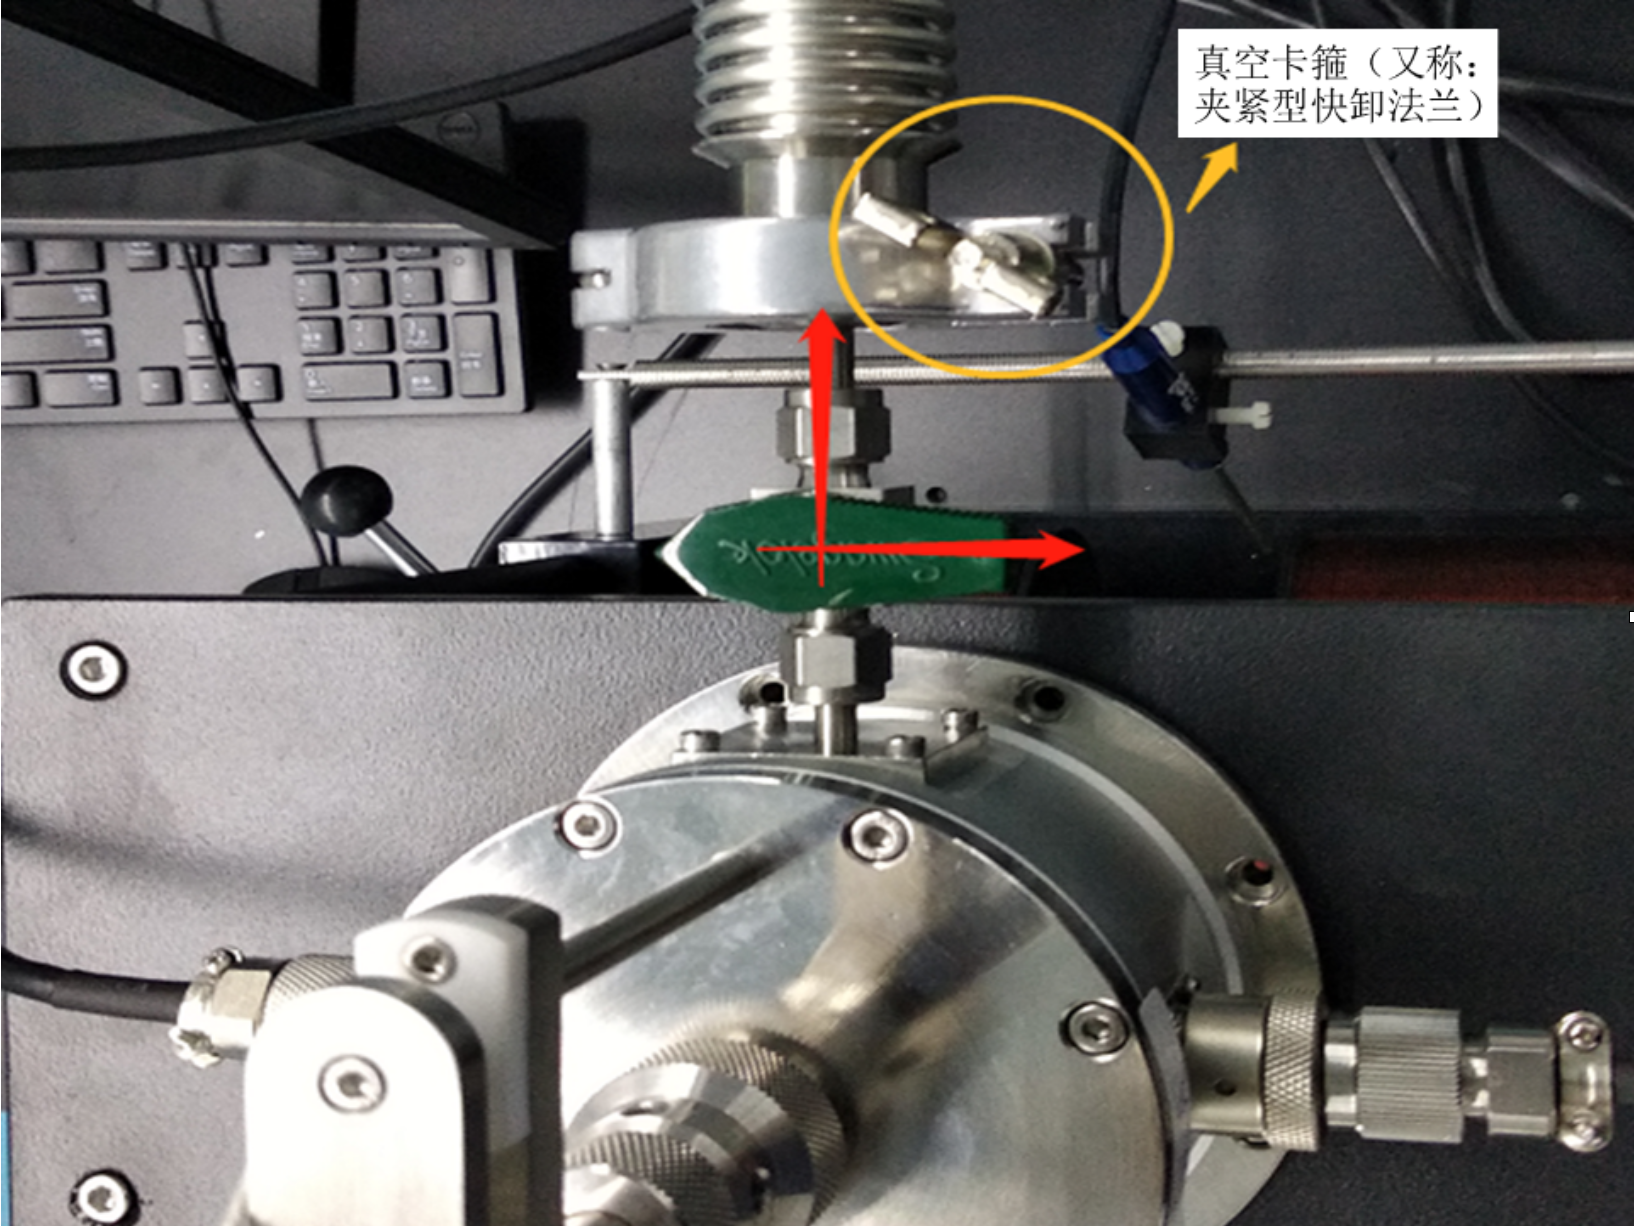
\includegraphics[width = 0.5\textwidth]{VacuumEntity.png}
                \end{figure}
                
            \subsubsection{设备电路连接}
                测量平台根据选择直流测量或交流测量而不同。
                \begin{longtable}{@{*}p{0.7\textwidth}||p{0.3\textwidth}@{*}}
                    \caption{设备电路连接操作步骤\label{tab:设备电路连接}}\\
                    \hline\hline
                    \multicolumn{1}{@{*}>{\centering}p{0.7\textwidth}||}{\textbf{操作}}&\textbf{完成情况}\\
                    \hline\hline
                    使用BNC连接恒温器与控温仪(六芯) & \\ \hline
                    连接恒温器与NI等测量平台 (八芯)& \\ \hline
                    连接恒温器、测量平台到电脑 & \\ \hline
                \end{longtable}
                
                \begin{figure}
                    \ct
                    \caption{恒温器设备线路连接图}
                    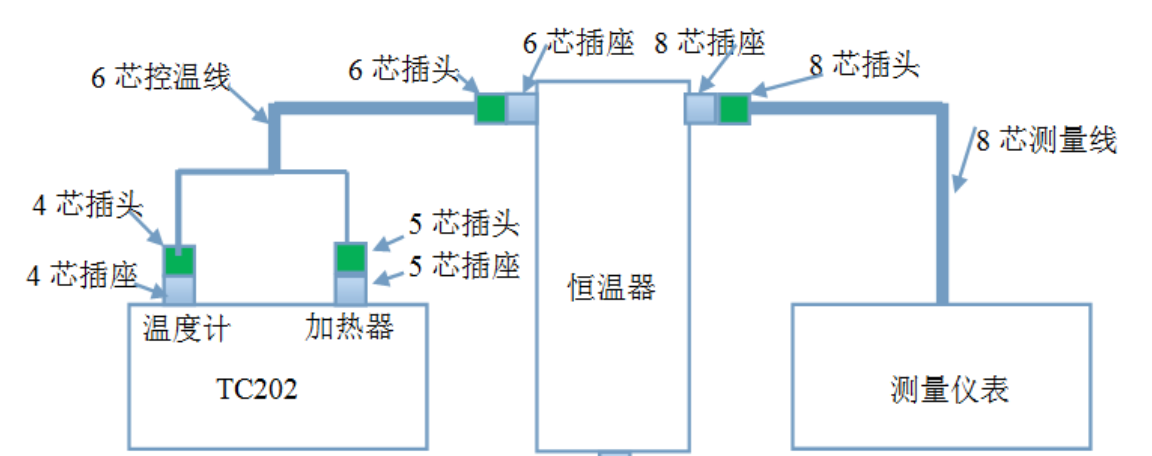
\includegraphics[width = 0.7\textwidth]{connection.png}
                \end{figure}

            \subsubsection{设备启动、预热}
                \begin{longtable}{@{*}p{0.7\textwidth}||p{0.3\textwidth}@{*}}
                    \caption{设备启动、预热操作步骤\label{tab:设备启动、预热}}\\
                    \hline\hline
                    \multicolumn{1}{@{*}>{\centering}p{0.7\textwidth}||}{\textbf{操作}}&\textbf{完成情况}\\
                    \hline\hline
                    打开NI机箱电源(前面板按钮) & \\ \hline
                    打开控温仪电源(前面板红色按钮) & \\ \hline
                    打开电磁铁电源(背后红色按钮,然后按前面板“power”长按3秒) & \\ \hline
                    打开OE4004电源预热 & \\ \hline
                    打开锁相放大器电源预热 & \\ \hline
                    打开普源数字多用表电源(先开后面板开关,再开前面板开关) & \\ \hline
                    打开电脑 & \\ \hline
                \end{longtable}
            
            \subsubsection{电脑程序与设备通讯}
                \begin{longtable}{@{*}p{0.7\textwidth}||p{0.3\textwidth}@{*}}
                    \caption{电脑程序与设备通讯操作步骤\label{tab:电脑程序与设备通讯}}\\
                    \hline\hline
                    \multicolumn{1}{@{*}>{\centering}p{0.7\textwidth}||}{\textbf{操作}}&\textbf{完成情况}\\
                    \hline\hline
                    打开电脑桌面LabView快捷方式“直流四引线测电阻”,检查设备连接 & \\ \hline
                \end{longtable}

            \subsubsection{液氮制冷}
                请熟悉液氮恒温器结构\autoref{img:液氮恒温器结构}与控温仪前面板\autoref{img:控温仪前面板}。控温过程控温仪负责控制加热速率,恒温器的中心塞控制制冷速率,两者合理调节
                才能或者较好的控温效果,请耐心调节。

                \begin{figure}
                    \ct
                    \caption{液氮恒温器结构}
                    \label{img:液氮恒温器结构}
                    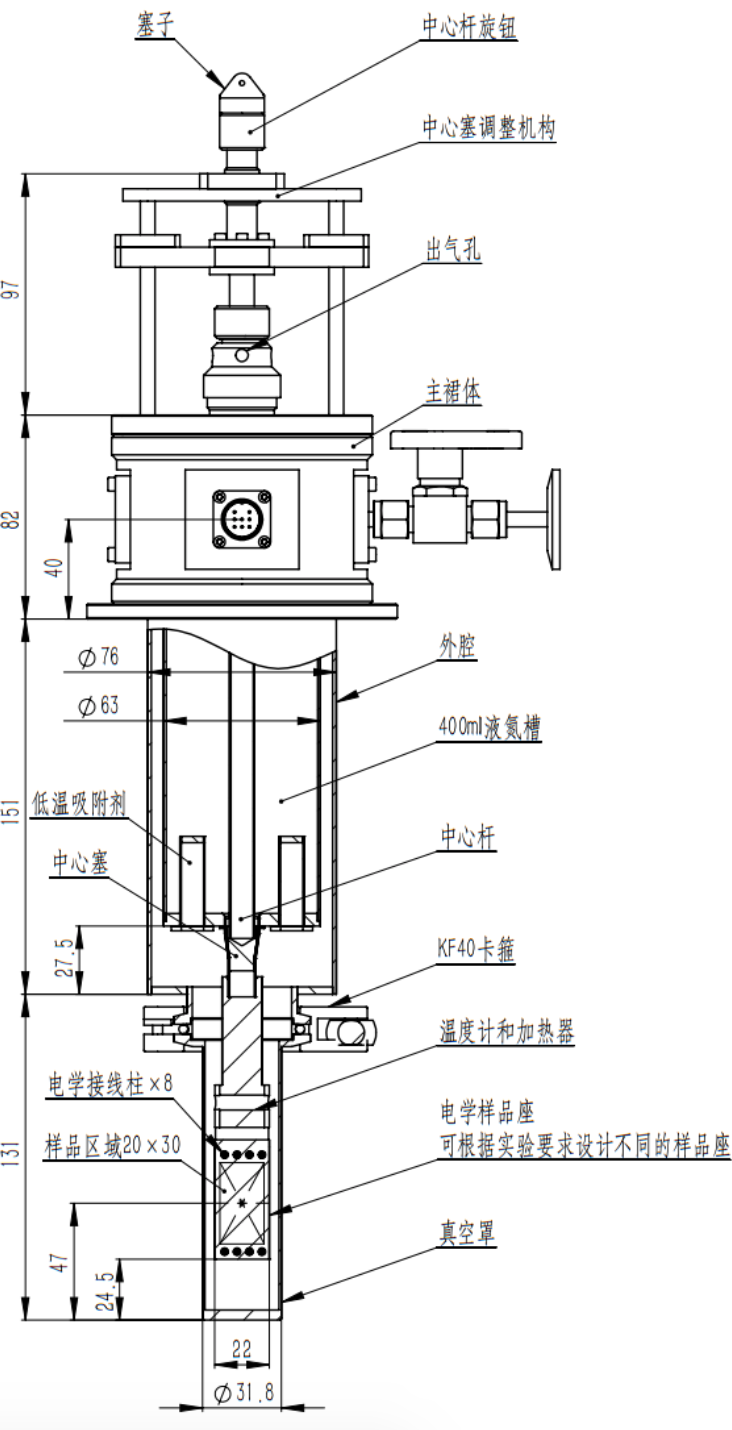
\includegraphics[width = 0.3\textwidth]{TempertureKeeper.png}
                \end{figure}
                \begin{figure}
                    \ct
                    \caption{控温仪前面板}
                    \label{img:控温仪前面板}
                    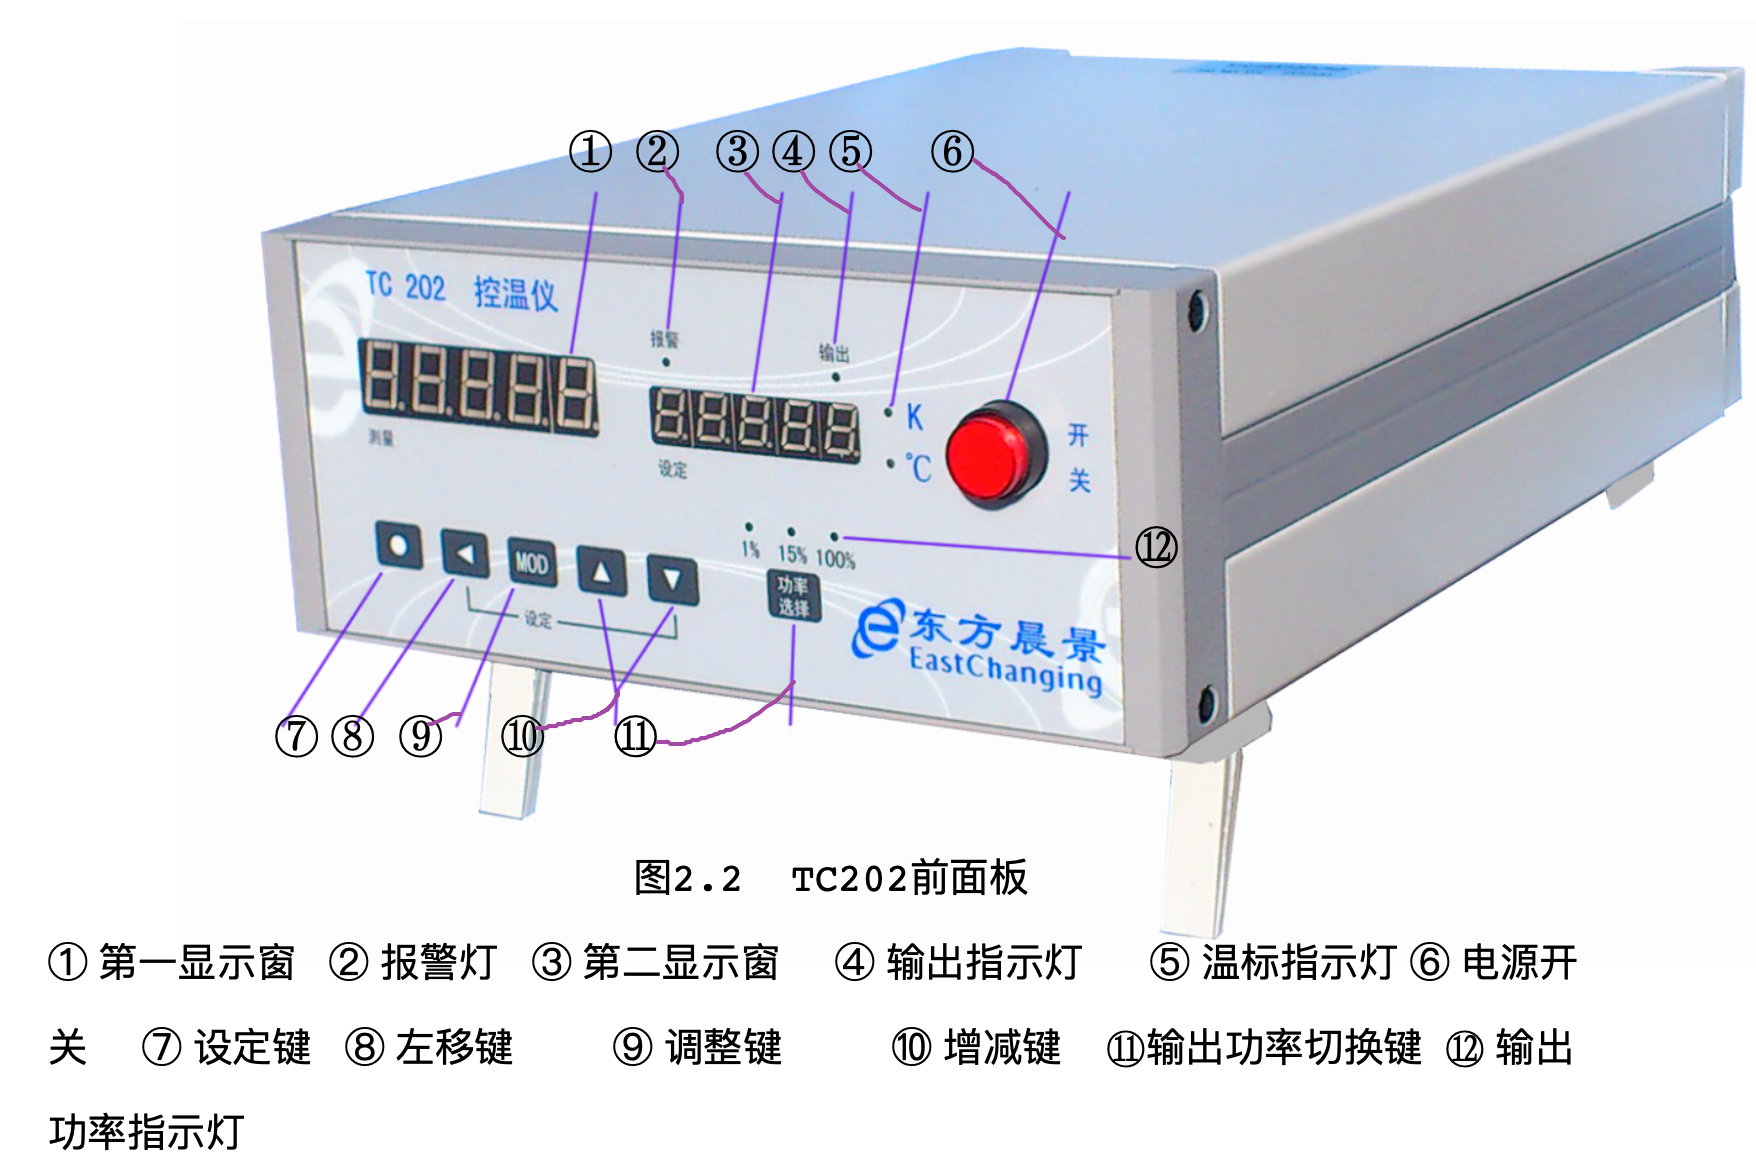
\includegraphics[width = 0.6\textwidth]{PIDFront.png}
                \end{figure}
                \at{1.5}
                \begin{longtable}{@{*}p{0.7\textwidth}||p{0.3\textwidth}@{*}}
                    \caption{液氮制冷操作步骤}\\
                    \hline\hline
                    \multicolumn{1}{@{*}>{\centering}p{0.7\textwidth}||}{\textbf{操作}}&\textbf{完成情况}\\
                    \hline\hline
                    真空抽取结束,关闭真空阀真空泵 & \\ \hline
                    顺时针旋转“中心杆旋钮”至旋转比较费劲,此时中心塞完全关闭,液氮不会会样品制冷 & \\ \hline
                    逆时针旋转两圈“中心杆旋钮”,此时中心塞处于中间位置。 可根据所需降温速率调节旋钮 & \\ \hline
                    检查注液漏斗是否有水珠,保持注液漏斗干燥 & \\ \hline
                    取下恒温器顶部的塞子,检查注入口附近是否干燥。 & \\ \hline
                    插入注液漏斗,操作人员站在远离“出气孔”的一侧,缓慢的加入液氮,以防液氮溅射冻伤操作人员。直到液氮有少量溢出,表明液氮已经加注满 & \\ \hline
                    使用纱布包住“出气孔”,防止水汽进入恒温器内部 & \\ \hline

                    \multicolumn{2}{c}{\textbf{设定控温仪}} \\ \hline \hline
                    控温仪通过自检后,第一个显示屏显示实测温度,第二显示屏显示目标控温温度 & \\ \hline
                    按前面板左键(8号键),目标控温温度的低位开始闪烁,此时用上下键(10号键)调节数值,再按左键切换调节位。设置目标控温为:XX K等待闪烁停止完成调节 & \\ \hline
                    观察第一个窗口实测温度的变化,根据控温速率调节加热功率,按“功率选择”按钮选择功率。只有当“报警灯”不亮,“输出灯“与”功率指示灯“同时亮时,控温仪才会有加热输出 & \\ \hline
                    非必要时勿调节控温器参数,若要调节请仔细阅读《控温仪TC202说明书》 & \\ \hline
                \end{longtable}
                \clearpage

        \subsection{制冷机制冷获得超导态(张旭盈、梁伟棠)}
    	
            \subsubsection{抽取真空}
                进行和液氮制冷相同的步骤,见\autoref{tab:抽取真空}。
            \subsubsection{设备电路连接}
                见\autoref{tab:设备电路连接}。
            \subsubsection{设备启动、预热}
                见\autoref{tab:设备启动、预热}。
            \subsubsection{电脑程序与设备通讯}
                见\autoref{tab:电脑程序与设备通讯}。
            \subsubsection{制冷机制冷}
                \begin{longtable}{@{*}p{0.7\textwidth}||p{0.3\textwidth}@{*}}
                \caption{制冷机制冷操作步骤}\\
                \hline\hline
                \multicolumn{1}{@{*}>{\centering}p{0.7\textwidth}||}{\textbf{操作}}&\textbf{完成情况}\\
                \hline\hline
                真空泵打开半个小时后开始制冷。先关闭真空阀,再关闭真空泵 & \\ \hline
                打开致冷机电源变压器(锁相放大器上方)开关,然后打开致冷机背后的电源开关 & \\ \hline
                1分钟后会听到冷头规律的马达声,表明致冷机正常启动,正常致冷速度起初约2K/min,后期降温速度逐渐变慢 & \\ \hline
                
                \multicolumn{2}{c}{\textbf{设定控温仪}} \\ \hline \hline
                控温仪通过自检后,第一个显示屏显示实测温度,第二显示屏显示目标控温温度 & \\ \hline
                按前面板左键(8号键),目标控温温度的低位开始闪烁,此时用上下键(10号键)调节数值,再按左键切换调节位。设置目标控温为:XX K等待闪烁停止完成调节 & \\ \hline
                观察第一个窗口实测温度的变化,根据控温速率调节加热功率,按“功率选择”按钮选择功率。只有当“报警灯”不亮,“输出灯“与”功率指示灯“同时亮时,控温仪才会有加热输出 & \\ \hline
                非必要时勿调节控温器参数,若要调节请仔细阅读《控温仪TC202说明书》 & \\ \hline
                适当注意观察压缩机氦气的压力,确保仪器工作正常。压缩机氦气压力表停机压力为1.7-2MPa,工作时压力略比正常高,大概在2MPa左右 & \\ \hline
                \end{longtable}

            \subsubsection{数据测量}
                需要通过测量样品的电阻或抗磁率,找到样品进入超导态的\textbf{转变温度}。
                \begin{longtable}{@{*}p{0.7\textwidth}||p{0.3\textwidth}@{*}}
                    \caption{第一次数据测量操作步骤}\\
                    \hline\hline
                    \multicolumn{1}{@{*}>{\centering}p{0.7\textwidth}||}{\textbf{操作}}&\textbf{完成情况}\\
                    \hline\hline
                    根据测量方案利用计算机进行测量值采集,输出测量记录并保存,记录文件名: & \\ \hline
                \end{longtable}

            \subsubsection{实验结束}
                测量完所需数据后,若需要拆开液氮恒温器改变实验则需要按照操作步骤结束恒温器的工作状态,不可暴力拆除。
                若改变的实验条件不需要拆开液氮恒温器如:加入磁场。则不需要结束恒温器工作状态。
                \begin{longtable}{@{*}p{0.7\textwidth}||p{0.3\textwidth}@{*}}
                    \caption{结束实验操作步骤}\\
                    \hline\hline
                    \multicolumn{1}{@{*}>{\centering}p{0.7\textwidth}||}{\textbf{操作}}&\textbf{完成情况}\\
                    \hline\hline
                    确定真空阀关闭状态,关闭真空泵 & \\ \hline
                    使用控温仪加热到290K稳定后,关闭控温仪及其他仪器 & \\ \hline
                    把所有连接线拆除,盖上恒温器塞子 & \\ \hline
                \end{longtable}
    \section{分析与讨论}
        \subsection{实验思考题}
        \begin{enumerate}
            \item 深低温系统为什么要抽真空?真空度要求多高?
            \begin{ans}
                在真空中热传导和对流可以忽略不计,只有热辐射传热,所以真空是一种很有效的隔热方式。真空度要求至多5Pa。
            \end{ans}

            \item 真空泵产生一定的噪声,在达到真空要求后,是否可以关真空泵?关真空泵前,是否要先关真空阀门?
            \begin{ans}
                可以关闭真空泵。先关真空阀,再关真空泵。
            \end{ans}
            
            \item 为什么要安装屏蔽罩(防辐射屏)?屏蔽罩用哪一类材料最好?
            \begin{ans}
                屏蔽罩可以有效减少热辐射传热。用导热性能较好的材料。
            \end{ans}

            \item 请估计直径为12mm、长为100mm,温度为4K的恒温器在无防辐射屏时的漏热约为多少?在采用一层防辐射屏后,其与环境之间的辐射漏热减少了多少?如果将防辐射屏的温度降到液氮温度(77K),则该防辐射屏的辐射漏热又为多少?
            \begin{ans}
                设室温为300K.默认题中所问是单位时间的漏热。
                无防辐射屏的漏热为:
                $\Delta Q_1 = \sigma(T_E^4 - T_L^4)St \\= 5.67032×10^{-8}W/(m^2·K^4)\times(300K^4-4K^4)\times(12mm\times100mm\times\pi+2\times(6mm/2)^2\times\pi)\times1s \\= 2.04\times10^{-5}J$
                采用防辐射屏后:
                $\Delta Q_2 =\frac12\Delta Q_1 = 1.02\times10^{-5}J$
                防辐射屏温度为77K时的辐射漏热:
            \end{ans}
   
            \item 铂电阻温度计位置不在样品旁边,有什么因素会影响样品温度偏离温度计的温度?偏离有多大?能否通过建模进行定量分析?
            \end{enumerate}

\end{document}